\documentclass[tikz,border=0mm]{standalone}
\usepackage{tikz}
\begin{document}

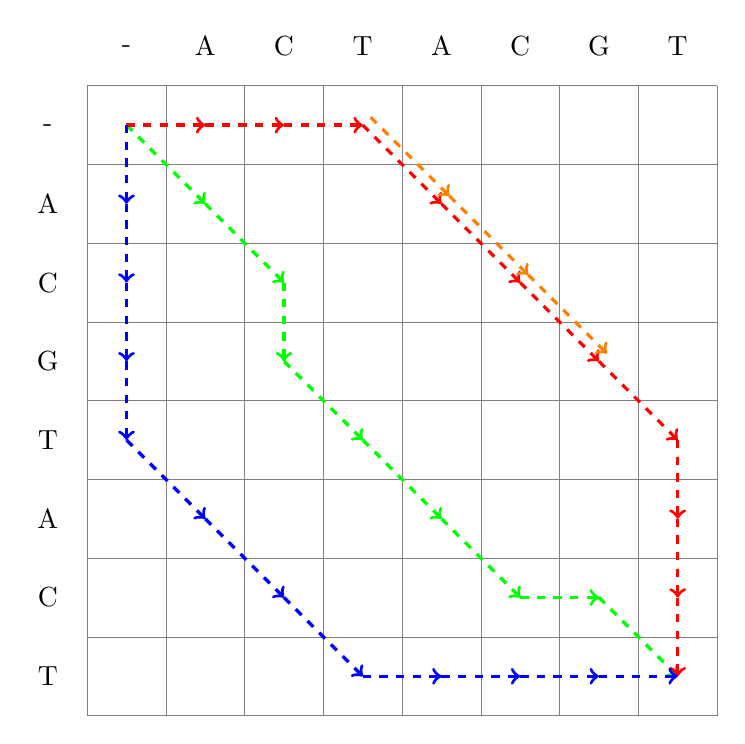
\begin{tikzpicture}
    \draw[step=1cm,gray,very thin] (0,-1) grid (8,7);

    % Labels for ACTACT
    \node at (-0.5, 6.5) {-};
    \node at (-0.5, 5.5) {A};
    \node at (-0.5, 4.5) {C};
    \node at (-0.5, 3.5) {G};
    \node at (-0.5, 2.5) {T};
    \node at (-0.5, 1.5) {A};
    \node at (-0.5, 0.5) {C};
    \node at (-0.5, -0.5) {T};
    
    % Labels for ACTACGT
    \node at (0.5, 7.5) {-};
    \node at (1.5, 7.5) {A};
    \node at (2.5, 7.5) {C};
    \node at (3.5, 7.5) {T};
    \node at (4.5, 7.5) {A};
    \node at (5.5, 7.5) {C};
    \node at (6.5, 7.5) {G};
    \node at (7.5, 7.5) {T};
    
    % First alignment
    \draw[green, very thick, dashed, ->] (0.5,6.5) -- (1.5,5.5);  % A -> A
    \draw[green, very thick, dashed, ->] (1.5,5.5) -- (2.5,4.5);  % C -> C
    \draw[green, very thick, dashed, ->] (2.5,4.5) -- (2.5,3.5);  % % Gap in first sequence (after C)
    \draw[green, very thick, dashed, ->] (2.5,3.5) -- (3.5,2.5);  % T -> T
    \draw[green, very thick, dashed, ->] (3.5,2.5) -- (4.5,1.5);  % A -> A
    \draw[green, very thick, dashed, ->] (4.5,1.5) -- (5.5,0.5);  % C -> C
    \draw[green, very thick, dashed, ->] (5.5,0.5) -- (6.5,0.5);  % Gap in second sequence (before T)
    \draw[green, very thick, dashed, ->] (6.5,0.5) -- (7.5,-0.5);  % T -> T
    
    % Second alignment
    \draw[red, very thick, dashed, ->] (0.5,6.5) -- (1.5,6.5);  % insert
    \draw[red, very thick, dashed, ->] (1.5,6.5) -- (2.5,6.5);  % insert
    \draw[red, very thick, dashed, ->] (2.5,6.5) -- (3.5,6.5);  % insert
    \draw[red, very thick, dashed, ->] (3.5,6.5) -- (4.5,5.5);  % A -> A
    \draw[red, very thick, dashed, ->] (4.5,5.5) -- (5.5,4.5);  % C -> C
    \draw[red, very thick, dashed, ->] (5.5,4.5) -- (6.5,3.5);  % G -> G
    \draw[red, very thick, dashed, ->] (6.5,3.5) -- (7.5,2.5);  % T -> T
    \draw[red, very thick, dashed, ->] (7.5,2.5) -- (7.5,1.5);  % delete
    \draw[red, very thick, dashed, ->] (7.5,1.5) -- (7.5,0.5);  % delete
    \draw[red, very thick, dashed, ->] (7.5,0.5) -- (7.5,-0.5);  % delete
    
    % Third alignment
    \draw[blue, very thick, dashed, ->] (0.5,6.5) -- (0.5,5.5);  % delete
    \draw[blue, very thick, dashed, ->] (0.5,5.5) -- (0.5,4.5);  % delete
    \draw[blue, very thick, dashed, ->] (0.5,4.5) -- (0.5,3.5);  % delete
    \draw[blue, very thick, dashed, ->] (0.5,3.5) -- (0.5,2.5);  % delete
    \draw[blue, very thick, dashed, ->] (0.5,2.5) -- (1.5,1.5);  % 
    \draw[blue, very thick, dashed, ->] (1.5,1.5) -- (2.5,0.5);  % 
    \draw[blue, very thick, dashed, ->] (2.5,0.5) -- (3.5,-0.5);  % 
    \draw[blue, very thick, dashed, ->] (3.5,-0.5) -- (4.5,-0.5);  % insert
    \draw[blue, very thick, dashed, ->] (4.5,-0.5) -- (5.5,-0.5);  % insert
    \draw[blue, very thick, dashed, ->] (5.5,-0.5) -- (6.5,-0.5);  % insert
    \draw[blue, very thick, dashed, ->] (6.5,-0.5) -- (7.5,-0.5);  % insert

    \draw[orange, very thick, dashed, ->] (3.6,6.6) -- (4.6,5.6);  % A -> A
    \draw[orange, very thick, dashed, ->] (4.6,5.6) -- (5.6,4.6);  % C -> C
    \draw[orange, very thick, dashed, ->] (5.6,4.6) -- (6.6,3.6);  % G -> G


    \end{tikzpicture}

\end{document}